\documentclass{article}

\usepackage{graphicx}
\usepackage[utf8]{inputenc}
\usepackage{url}
\usepackage{multirow,tabularx}
\usepackage{subcaption}

\usepackage{listings}
\renewcommand{\ttdefault}{pcr} % Courier instead of Computer Modern
% Fix dashes in listings (from
% https://tex.stackexchange.com/questions/33185/listings-package-changes-hyphens-to-minus-signs
% )
\makeatletter
\lst@CCPutMacro\lst@ProcessOther {"2D}{\lst@ttfamily{-{}}{-{}}}
\@empty\z@\@empty
\makeatother
\lstdefinelanguage{Futhark}
{keywords={fun,if,then,else,loop,do,map,Map,Red,reduce,reduceComm,filter,scan,redomap,redomapComm,transpose,rearrange,reshape,iota,replicate,let,in,for,while,with,f32,int,zip,streamSeq,zipWith,unsafe,streamRed,streamMap,mapPerThread,fn,reduceKernel,concat,split,size,local},%
  sensitive=true,
  comment=[l]{--},
  moredelim=**[is][\color{red}]{@}{@},
  moredelim=**[is][\color{blue}]{!}{!},
}

\lstset{
  language=Futhark,
  basicstyle=\ttfamily\small,
  keywordstyle=\bfseries,
  showlines=true,
  columns=fullflexible,
  keepspaces=true,
}

\title{Improving Performance of Part of LexiFi's Heston Calibration
  via a port from OCaml to Futhark}

\author{Troels Henriksen}

\begin{document}

\maketitle

  \begin{abstract}
    This technical report describes the porting of LexiFi's Heston
    Calibration Model from OCaml to Futhark, with the goal of
    obtaining significant performance improvements via parallel
    execution.  The close similarity between OCaml and Futhark, both
    high-level languages in the ML family, enabled a mostly
    straightforward translation, although some changes in coding style
    were effected to take full advantage of Futhark.  The resulting
    program runs from $76\times$ to $428.02\times$ faster than the
    original OCaml code, and there is potential for further
    performance improvements.  This work suggests that Futhark
    provides a potential for dramatic performance improvements, while
    keeping the source code as readable as OCaml.

    This project was hosted by SimCorp Technology Labs.
  \end{abstract}

\section{Introduction}

Instrument Box is a library of financial algorithms marketed by the
French company LexiFi.  This library is used at the Danish company
SimCorp, and is often referred to as \textit{mlfi}.  The Instrument
Box is written in OCaml, an expressive functional language in the ML
family.  While OCaml is well regarded for the the quality of the
sequential code emitted by its compiler, it is unable to take
advantage of modern high-performance parallel execution platforms,
such as vectorised CPUs or GPUs.  As current and future improvements
in hardware performance tend to come in the form of increased
parallelism, this will present scaling problems if users become
interested in applying the algorithms to increasingly larger data
sizes.

This document summarises a two-month period during which I have
investigated the use of
\textit{Futhark}\footnote{\url{https://futhark-lang.org}} to enable
parallel execution of selected algorithms from the Instrument Box.
Futhark is a high-performance functional array language developed as
part of the HIPERFIT\footnote{\url{http://hiperfit.dk}} project at the
computer science department at the University of Copenhagen.  It is a
high-level and platform-agnostic language, similar to OCaml in both
syntax and semantics, but with restrictions (and some extensions) to
enable efficient execution on parallel machines.  The hypothesis is
that Futhark can enable efficient parallel execution of programs that
are close to their original OCaml formulation, while shielding the
programmer from having to know intricate details of parallel hardware.
The ambition is not to match the performance of hand-tuned low-level
code written by experts, but to provide a balance between high-level
code and low-level performance.  Concretely, Futhark uses the
standardised OpenCL API to orchestrate execution on GPUs and
multi-core CPUs.

This project is a continuation of previous collaboration between
HIPERFIT and LexiFi on high-performance methods, where kernels for
interest rate calibration and local volatility calibration have been
manually ported and tuned for multi-core CPU and many-core GPU
execution~\cite{FinPar:TACO}.  In contrast to this previous work, which
focused mostly on parallel performance potential inherent in the
financial algorithms, I have attempted to stay closer to the
formulations in the original implementations.  With this report, I
seek to answer three concrete questions:

\begin{enumerate}
\item What is the potential for runtime improvement by parallelising
  computational kernels, and what has been achieved?

\item Is Futhark expressive enough to handle the algorithms from
  LexiFi, what is the effort required to translate LexiFi's OCaml/C to
  Futhark, and how similar is the resulting code to the original?

\item If a transpiler from OCaml to Futhark existed and given the
  implementation of the algorithm made in Futhark as output of the
  said transpiler, what would the input OCaml code look like?
\end{enumerate}

Answers are given in Section~\ref{sec:conclusions}.
Section~\ref{sec:overview} describes the background of the work, and
technical details are provided in Section~\ref{sec:implementation}.
Invaluable assistance has been provided by Olivier Pradère from
LexiFi.

\section{The Problem}
\label{sec:overview}

The investigation has proceeded by porting from OCaml to Futhark a
subset of a calibration routine for the Hybrid Stochastic Local
Volatility / Hull-White model (SLV HW model).  This routine has been
extracted from the full Instrument Box library, with the main
modification being that a sub-component has been translated from C to
OCaml by LexiFi.  We will refer to the OCaml version as the
\textit{reference implementation}.  Only a subset, comprising
\textit{pure Heston}~\cite{mikhailovheston} calibration, has been
ported to Futhark.

As I am not an expert in financial mathematics, I have not explored
algorithmic improvements during the project.  It is conceivable that
there exists an alternative to this calibration algorithm that is
better suited to parallel execution, but I have taken the
implementation as given, and simply tried to accelerate it via porting
to Futhark.

The calibration routine takes as its main input a series of observed
\textit{quotes}.  A quote is a triple consisting of a maturity date, a
strike price, and a quote price.  The model attempts to determine five
Heston parameters that match the observed quotes, with the intent that
these parameters can then be used to price other quotes in the Heston
model.

The fitting of the five Heston parameters is carried out in a fairly
conventional manner.  Least-squares optimisation is used via the
Differential Evolution algorithm~\cite{Storn1997}, where the objective
function performs closed-form pricing of European options in the
Heston model.  Intuitively, the algorithm is an evolutionary (or
``genetic'') algorithm that proceeds by maintaining a
\textit{population} of candidate parameters, which are repeatedly
randomly perturbed.  The random modifications that result in the most
improvement (judged via the objective function) are then chosen for
further evolution.  It is thus hard for a re-implementation to match
the reference implementation \textit{exactly}, as it is sensitive to
how the randomness is generated.  Furthermore, there is no
\textit{single} correct result, as the only measure of algorithmic
success is how well the final parameters minimise the error in the
objective function.  However, as long as a re-implementation is able
to generate results of approximately the same quality as the reference
solution, it can be considered correct.

In the original Instrument Box implementation, the least-squares
procedure is a sequential C program (\texttt{mpfit}~\cite{0902.2850},
which is itself a port of an older Fortran program~\cite{More1978}).
In the extracted routine used as the reference for this project,
\texttt{mpfit} has been replaced with a least-squares implementation
written in pure OCaml.  It is likely that the OCaml implementation is
somewhat slower than \texttt{mpfit}, although I have not measured to
which degree.

\section{Implementation}
\label{sec:implementation}

The Futhark implementation comprises three main parts: (i) a
general-purpose least-squares implementation using the Differential
Evolution algorithm, (ii) a European call pricer, and (iii) the
integration between the first two (plus a slight amount of
preprocessing).  The vast amount of the run-time work takes place
inside the least-squares solver, which uses the European call pricer
as the objective function.  Thus, this is the part on which I will
focus.

During the implementation, I have attempted to preserve the structure
and intent of the original code.  The three parts listed above are
just as decoupled as in the reference implementation.  For example,
the least-squares implementation is \textit{generic} in its choice of
objective function, even though we only ever apply to the European
call pricer.  It is possible that better performance could be achieved
by writing a tight coupling between the solver and the objective
function, but at a significant cost in readability and capacity for
re-use.

When describing the implementation and its performance
characteristics, I will refer to input sizes by the names of variables
in the Futhark implementation.  These are similar to the corresponding
names in the OCaml implementation, but are used more consistently.

The program contains several parallel loops enclosed within each
other, as shown on Figure~\ref{fig:loopstructure}.  This kind of
parallel structure is called \textit{nested parallelism}, and is in
the general case notoriously difficult to compile to efficient
code~\cite{blelloch1994implementation}.  The parameters controlling
the number of iterations of the parallel loops are as follows:

\begin{description}
\item[\texttt{num\_free\_vars}:] The number of parameters that we are
  fitting.  For the Heston model, this is always $5$.
\item[\texttt{np}:] The population size used for the Differential
  Evolution algorithm.  The reference limitation sets this to times
  the number of variables to fit (\texttt{num\_free\_vars}), but with
  an upper bound of $40$.  This has been maintained in the Futhark
  implementation.
\item[\texttt{num\_quotes}:] The number of observed quotes.  In
  practice, this is the quantity that can vary between data sets, and
  thus the only scalable source of parallelism.  However, while it is
  easy to synthesise a large set of quotes, is is unclear how large
  this array is in realistic workloads.
\item[\texttt{num\_points}:] The number of Gauss-Laguerre coefficients
  used for pricing options in the objective function.  This is either
  $20$ or $10$, but always set to $20$ in the reference
  implementation, which I have followed in the Futhark
  implementations.
\end{description}

Many parallel libraries and languages simply do not support nested
parallelism at all.  However, this particular algorithm exhibits
\textit{regular} nested parallelism, in which the number of iterations
performed by an inner loop does not depend on an outer loop.  Regular
nested parallelism is much easier to compile efficiently, and is
handled by the Futhark compiler.

The parallel loops are repeatedly executed by the sequential outer
\texttt{while}-loop until a \textit{convergence criterion} is reached.
The convergence criterion is configurable, and can be either reaching
a specified error tolerance, a given number of iterations, or a number
of calls to the objective function.  For the Heston model, the error
tolerance is set to zero and the maximum number of iterations to
$2^{31}-1$.  The maximum number of calls to the objective function is
dataset-specific, but is $2000$ for all data sets used for this
project.  In practice, this is the limit that we will reach.  Note
that the convergence loop invokes the objective function exactly
\texttt{np} times for each iteration.

\begin{figure}
  \centering
  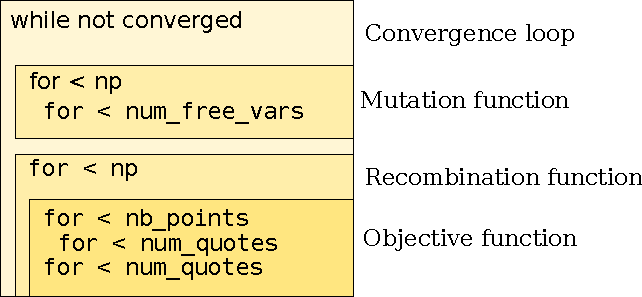
\includegraphics{loopstructure.pdf}
  \caption{Loop Structure of the Heston Calibration Program.
    Indentation shows the nesting of loops.  All loops are parallel,
    except for the outer convergence loop.  Some loops involve
    reductions, while others are fully independent.  The coloured
    boxes and their labels indicate the logical structure of the
    code.}
  \label{fig:loopstructure}
\end{figure}

\section{Performance}

I compare the runtime of the Futhark implementation to the reference
implementation on three data sets: one with $1062$ quotes, one with
$10,000$ quotes, and one with $100,000$ quotes.  The latter two are
synthetic, but the first data set is representative of the scale of
the typical inputs used in practice.  The Futhark implementation has
been executed in parallel on both an NVIDIA K40 GPU (commonly used for
compute tasks), as well as on a multi-core Intel laptop CPU. The
resulting runtimes are shown on Table~\ref{tab:runtimes}.

Runtime measurements for parallel execution do not include OpenCL/GPU
driver initialisation or kernel compilation, nor does it include
copying initial input to the device.  The time taken for this copying
is negligible compared to the overall runtime.

\textit{Speedup} for a given dataset and platform is computed by
comparing the achieved runtime to the best runtime of the reference
implementation on the same dataset.  This is the number that indicates
how much faster the Futhark implementation is than reference
implementation.  Note that the CPU used to obtain the fastest OCaml
execution is not the same as the CPU used to run parallel Futhark
code.

It is unsurprising that GPU speedup is significantly lower on the
smallest dataset ($1062$ quotes), as this dataset contains
insufficient parallelism to amortise the overhead of parallel
execution on a GPU.  Figure~\ref{fig:speedups} shows the relationship
between input size and speedup for GPU execution.  Parallel CPU
execution is less dependent on large amount of parallelism, and hence
shows stable speedup for all input sizes.

\begin{table}
  \centering
\begin{tabular}{l|l|r|r}
  \textbf{Dataset} & \textbf{Platform} & \textbf{Runtime} & \textbf{Speedup} \\\hline\hline

  \multirow{2}{*}{$\texttt{num\_quotes}=1062$} & Core i5-5300 (OCaml; sequential) & $4.60s$ & $1.00\times$ \\
  & Core i5-5300 (Futhark; sequential) & $4.12s$ & $1.12\times$ \\\hline
  \multirow{2}{*}{$\texttt{num\_quotes}=10,000$} & Core i5-5300 (OCaml; sequential) & $38.54s$ & $1.00\times$ \\
  & Core i5-5300 (Futhark; sequential) & $27.95s$ & $1.38\times$  \\\hline
  \multirow{2}{*}{$\texttt{num\_quotes}=100,000$} & Core i5-5300 (OCaml; sequential) & $441.60s$ & $1.00\times$ \\
  & Core i5-5300 (Futhark; sequential) & $298.39s$ & $1.48\times$ \\\hline

  \multirow{3}{*}{$\texttt{num\_quotes}=1062$} & Core i5-4300 (Futhark; sequential) & $8.99s$ & $0.50\times$ \\
  & Core i5-4300 (Futhark; four cores) & $0.55s$ & $8.36\times$ \\
  & NVIDIA Tesla K40 (Futhark) & $0.06s$ & $76.7\times$ \\\hline

  \multirow{3}{*}{$\texttt{num\_quotes}=10,000$} & Core i5-4300 (Futhark; sequential) & $79.47s$ & $0.50\times$ \\
  & Core i5-4300 (Futhark; four cores) & $4.34s$ & $8.88\times$ \\
  & NVIDIA Tesla K40 (Futhark) & $0.24s$ & $160.6\times$ \\\hline


  \multirow{3}{*}{$\texttt{num\_quotes}=100,000$} & Core i5-4300 (Futhark; sequential) & $852.38s$ & $0.50\times$ \\
  & Core i5-4300 (Futhark; four cores) & $47.85s$ & $9.23\times$ \\
  & NVIDIA Tesla K40 (Futhark) & $2.22s$ & $198.92\times$ \\
\end{tabular}
  \caption{Runtimes of reference and Futhark implementation on various platforms.  Speedups are relative to the fastest reference runtime for a given dataset.}
  \label{tab:runtimes}
\end{table}

\begin{figure}
  \centering
  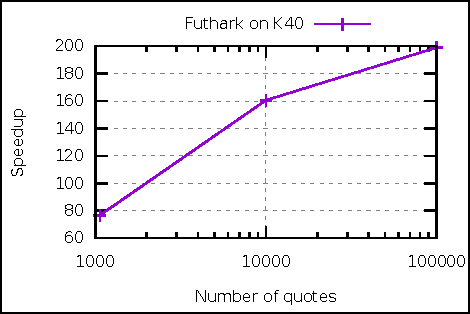
\includegraphics{speedup.pdf}
  \caption{Visualisation of Speedup on K40 GPU}
  \label{fig:speedups}
\end{figure}

\subsection{Performance Potential}

An estimate of the potential peak performance for this program can be
estimated by measuring the \textit{arithmetic intensity}.  The
arithmetic intensity is the ratio of total floating-point operations
to total data movement.  The generated GPU code is dominated by the
runtime of three primary kernels (corresponding to parallel sections
of the least-squares convergence loop), for which I have manually
estimated the arithmetic intensity by counting instructions
(Table~\ref{tab:arithmetic-intensity}).  We can compute the arithmetic
intensity of the overall application by weighting these measurements
by the proportion of runtime spent in each of the three kernels, which
comes out to $0.47$.  Similarly, by counting number of floating point
operations divided by the kernel runtimes (not shown here), the
weighted total floating-point throughput can be computed as $68.57$
GFLOPS.  This estimate treats all floating-point operations as equal,
even though some (such as arc tangent) may be more expensive than
others.  All numbers used in this section have all been obtained by
running on the largest data set ($100,000$ quotes).

The GPU used (an NVIDIA Tesla K40) has peak double-precision of
performance of around $1310$ GFLOPS, but only $250$GiB/s of memory
bandwidth, and thus requires an arithmetic intensity of around $5.26$
in order for performance to be compute-bound.  At the arithmetic
intensity exhibited by the program, we can expect no more than
$116.98$ GFLOPS.  It is clear that the best further avenue of
optimisation is to make more efficient use of memory.  Note also that
the K40 GPU used is a fairly old model, and the newer Pascal GPUs have
approximately four times as much memory bandwidth available.

\begin{table}
  \centering
  \begin{tabular}{l|r|r|r}
    \textbf{Kernel} & \textbf{Runtime fraction} & \textbf{Arithmetic intensity} & \textbf{FLOPS} \\\hline\hline
    A & $0.47$ & $0.62$ & $72.50$ GFLOPS \\
    B & $0.35$ & $0.16$ & $78.47$ GFLOPS \\
    C & $0.17$ & $0.74$ & $41.37$ GFLOPS \\
  \end{tabular}
  \caption{Arithmetic intensity of the three main GPU kernels and of
    the overall application, as well as the achieved FLOPS.}
  \label{tab:arithmetic-intensity}
\end{table}

\subsection{Using Single-Precision Floating Point}

As the previous section shows, the Heston Calibration program is
bandwidth-bound.  An immediate avenue of optimisation is thus to
investigate ways to reduce the memory traffic.  The reference
implementation uses double-precision floating point numbers for all
calculations.  This is likely because this is the default of the OCaml
\texttt{real} type, but also because there is little difference in
performance between single and double-precision numbers on CPUs.  On
GPUs, however, the fact that single-precision numbers take up only 32
bits of space instead of 64 bits for double-precision numbers, mean
that programs using single-precision are often significantly
faster.\footnote{Many GPUs are also further crippled in
  double-precision performance for reasons of market segmentation, but
  that is not the case for the Tesla K40 used for the benchmarks in
  this paper.}.  In fact, if we assume that all memory traffic
consists of floating-point numbers, then switching to single-precision
should cut the memory traffic (and runtime) in half.

The Futhark implementation has been written using generic programming
techniques, making it easy to switch between double to single
precision without having to maintain two separate programs.
Table~\ref{tab:single-precision} reproduces the runtimes for the
double-precision implementation on GPUs, and also shows the runtimes
and speedups (again compared to the reference implementation) for a
single-precision version.  The impact is substantial - more than a
factor of two.  This is likely a combination of reduced memory
traffic, but also lower register pressure, permitting more threads to
execute concurrently.

\begin{table}
  \centering
\begin{tabular}{l|l|r|r}
  \textbf{Dataset} & \textbf{Platform} & \textbf{Runtime} & \textbf{Speedup} \\\hline\hline

  \multirow{2}{*}{$\texttt{num\_quotes}=1062$} & NVIDIA Tesla K40 (doubles) & $0.06s$ & $76.70\times$ \\
  & NVIDIA Tesla K40 (singles) & $0.04s$ & $115.05\times$ \\\hline

  \multirow{2}{*}{$\texttt{num\_quotes}=10,000$} & NVIDIA Tesla K40 (doubles) & $0.24s$ & $160.60\times$  \\
  & NVIDIA Tesla K40 (singles) & $0.12s$ & $321.20\times$ \\\hline

  \multirow{2}{*}{$\texttt{num\_quotes}=100,000$} & NVIDIA Tesla K40 (doubles) & $2.22s$ & $198.92\times$ \\
  & NVIDIA Tesla K40 (singles) & $1.03s$ & $428.02\times$ \\
\end{tabular}
\caption{Comparing the performance of using double precision versus
  single precision floating-point numbers.}
  \label{tab:single-precision}
\end{table}

Switching from double to single-precision numbers is not without its
downsides.  Single-precision numbers are substantially less accurate,
and the calibration results produced by the single-precision version
are not as good as those produced by the double-precision version.
For example, on the $\texttt{num\_quotes}=100,000$ dataset, the
double-precision version produces a result with a root-mean-square
error of $0.2$, while the single-precision version produces a result
with a root-mean-square error of $0.3$.  However, if we permit the
single-precision version to calibrate for twice as many iterations
($4000$ instead of $2000$), it still runs slightly faster than the
double-precision version, and produces a result with root-mean-square
error of $0.08$.  This shows that judicuous use of single-precision
numbers can lead to simultaneously better performance and equivalent
or better calibration results.

\section{Porting Challenges}

While the final Futhark implementation resembles the original OCaml
implementation and performs well, several challenges had to be
overcome to get to that point.  Some of these could be resolved by
extending or improving the Futhark language and compiler, while others
require more long-term work to resolve, and have in the short term
been handled with local workarounds.  I believe that the challenges I
encountered will be representative of what can be expected from future
ports of LexiFi OCaml to Futhark (albeit hopefully encountering fewer
bugs in the Futhark compiler).

\subsection{Record Types}

At the start of the project, Futhark did not have support for record
types.  While record types are in principle merely syntactical sugar
on top of tuples, they can drastically improve readability.  As a
result, some time was spent adding record types to Futhark, which
enabled the Futhark implementation to match the reference
implementation much more closely.

\subsection{First-Class Functions}

OCaml, as a functional language in the style of $\lambda$-calculus,
supports fully first-class functions, that is, functions that can be
used as values.  Futhark is a language designed for compilation to
highly performant code, and as first-class functions are difficult to
compile and optimise efficiently (especially on GPUs), they are not
supported.

For the most part, the reference implementation uses first-class
functions only in a very limited way, namely to define
\textit{higher-order functions} (functions accepting functions as
parameters).  For example, the least-squares implementation is
parameterised over the objective function, which is passed as a
parameter of type \texttt{('a -> float array -> unit)}.  This usage
can be modeled via the use of \textit{higher-order modules} instead.
Higher-order modules are a sophisticated (and slightly esoteric)
feature by which modules can be parameterised over another module.
Essentially, they are functions at the module level, which can be
evaluated statically during compilation.  Higher-order modules are
typically found in ML-style module systems, and are supported by both
Futhark and OCaml.  In the future, it is likely that Futhark will gain
limited support for polymorphic higher-order functions, such that
using the module system as a workaround becomes unnecessary.

In a few places, higher-order functions are used more liberally by the
reference implementation.  For example, the \texttt{least\_squares}
function in \texttt{optimization.ml} uses a (morally) boolean
parameter to select between two different norm functions.  A snippet
is shown on Figure~\ref{fig:fcf-example}.  Such uses involve a little
more refactoring, in this case by making the norm function a parameter
directly, instead of picking it based on a branch.

\begin{figure}
  \centering
\begin{lstlisting}[language=Caml]
let norm = match absolute with
  | None -> fun acc price quote ->
              let rel = (price -. quote) /. quote in acc +. rel *. rel
  | Some() -> fun acc price quote ->
                let dif = price -. quote in acc +. dif *. dif
\end{lstlisting}
  \caption{An example use of first-class functions in the reference
    implementation, in which a boolean parameter is used to
    select between two norm functions.}
  \label{fig:fcf-example}
\end{figure}

\subsection{Sequential to Parallel Loops}

As a functional language, OCaml supports the usual repertoire of
higher-order looping functions such as \texttt{map} and
\texttt{reduce}.  However, the reference implementation is written
with pervasive use of imperative loops and in-place updates of arrays.
This is for performance reasons, as the OCaml compiler is known to
generate very efficient machine code for OCaml written in a
conventional procedural style.

Unfortunately, the procedural coding style hides the parallelism
inherent in the original algorithm.  In the Futhark implementation,
these loops have been rewritten using \texttt{map} and \texttt{reduce}
combinators.  As an example, the OCaml and Futhark code for the
recombination loop is shown on Figure~\ref{fig:loop-comparison}.  The
recombination loop evaluates the objective function (\texttt{f}) on
every element of \texttt{f}.  For each such evaluation (stored in
\texttt{f\_v}), it is checked whether the result is better than the
previous best result for the population (\texttt{fx.(i)}), and if so,
the new result is stored.  It is also checked whether the new result
is better than the globally best result (\texttt{fx0}), and if so,
\texttt{best\_idx} is updated to point at it.

The two code snippets compute essentially the same: new values for
\texttt{fx0}, \texttt{best\_idx}, \texttt{fx}, and \texttt{x}.  In the
OCaml code on Figure~\ref{fig:ocaml-loop}, this is done with an
imperative loop (through the library function \texttt{Array.iteri}).
The loop body performs updates of array elements (the \texttt{x} and
\texttt{x0} arrays), as well as the mutable variables \texttt{fx0} and
\texttt{best\_idx}.  The loop iterations are not independent, as they
read and write to the same variables.

In the Futhark code on Figure~\ref{fig:futhark-loop}, the
recombination loop has been written using the parallel combinators
\texttt{map} and \texttt{reduce\_comm} (commutative reduction).  Four
parallel loops are used, but the compiler employs automatic
\textit{loop fusion} to combine them into just one loop.  The coding
style used here is typical of data-parallel functional programming,
where the focus is on \textit{bulk operations}, rather than moving
around single scalar values.  Also, the Futhark program returns its
result as \textit{fresh} values, while the OCaml program modifies
existing arrays and variables.

None of the constructs used in the Futhark implementation should be
unfamiliar to an OCaml programmer, and OCaml could easily be written
in the same style, although likely with a performance penalty.

\begin{figure}
  \centering
  \begin{subfigure}{1\textwidth}
\begin{lstlisting}[language=Caml]
let recombination () =
  Array.iteri
    (fun i v_i ->
       let f_v = f v_i in
       if f_v < fx.(i) then begin
         fx.(i) <- f_v;
         Array.blit v_i 0 x.(i) 0 n;
         if f_v < !fx0 then begin
           best_idx := i;
           fx0 := f_v;
           call_back !ncalls f_v;
           Array.blit v_i 0 x0 0 n
         end;
       end;
    ) v
\end{lstlisting}
    \caption{OCaml}
    \label{fig:ocaml-loop}
  \end{subfigure}

  \begin{subfigure}{1\textwidth}
\begin{lstlisting}
let recombination (fx0: real) (best_idx: i32)  (fx: [np]real)
                  (x: [np][num_free_vars]real) (v: [np][num_free_vars]real) =
  let f_v = map f v
  let fx' = map real.min f_v fx
  let x' = map (\f fx_i x_i v_i -> if f < fx_i then v_i else x_i)
               f_v fx x v
  let (fx0', best_idx') =
    reduce_comm min_and_idx
                (fx0, best_idx)
                (zip (intrinsics.opaque f_v) (iota np))
  in (fx0', best_idx', fx', x')
\end{lstlisting}
    \caption{Futhark}
    \label{fig:futhark-loop}
  \end{subfigure}
  \caption{Comparison of sequential OCaml loop to corresponding parallel Futhark loop}
  \label{fig:loop-comparison}
\end{figure}

\subsection{Exploiting Nested Parallelism}

As shown on Figure~\ref{fig:loopstructure}, the Heston calibration
algorithm contains several layers of parallelism.  In a nested
parallel program, there is no \textit{single best way} to exploit the
available parallelism.  The objective is to exploit as much as is
needed to saturate the machine on which we are running, but
\textit{excess parallelism} often comes with significant overhead.
For example, a nested \textit{reductions} (such as a summation) can be
parallelised, or left as a sequential loop inside a parallel thread.
The latter is more efficient if we do not need the extra parallelism.
However, a compiler knows only \textit{symbolic} sizes, and thus
cannot (in general) decide the optimal parallelisation structure at
compile-time.  Currently, the Futhark compiler uses built-in
\textit{heuristics} to decide how to exploit available parallelism,
but these are often wrong.

For the data sets used to benchmark the Heston calibration, the
optimal parallelisation structure is to fully parallelise the mutation
function.  For the recombination function, the \texttt{np} loop level
should be parallelised, while the \texttt{nb\_points} and
\texttt{num\_quotes} loops should be interchanged, and the
\texttt{nb\_points} loop sequentialised.  Workaround have been added
to the Futhark implementation to guide the compiler heuristics towards
making these choices.  However, this would not be the optimal choice
for a hypothetical data set where \texttt{num\_quotes} is small and
\texttt{nb\_points} is large.

This is a known problem for nested parallelism, and a future Futhark
research topic is to remove the need for such workarounds.  Our
intended solution is \textit{multi-versioned code}, where \textit{all}
feasible parallelisation structures are generated, and the optimal one
selected at run-time, based on input data characteristics.

\section{Conclusions}
\label{sec:conclusions}

\paragraph{What is the potential for runtime improvement by
  parallelising computational kernels, and what has been achieved?}

Parallelising the Heston calibration yields speedups over sequential
execution ranging from $76\times$ to $198\times$, with larger datasets
yielding better speedup.  The smallest dataset (which yields a
$76\times$ speedup) is representative of current usage, which
therefore establishes a lower bound on practical achievable speedup.

The achieved speedups are likely well below the full potential.  The
Futhark implementation executes on a K40 GPU at an estimated $68.57$
GFLOPS, compared to the $116.98$ that are theoretically possible given
the arithmetic intensity of the algorithm.  Optimisations to lower
memory traffic requirements would increase the arithmetic intensity of
the program, and likely result in significant speedup.

The results also show that the Futhark implementation performs
excellently on a commodity laptop CPU, suggesting that GPUs are not
the only way to obtain acceleration of this program.

\paragraph{Is Futhark expressive enough to handle the algorithms from
  LexiFi, what is the effort required to translate LexiFi's OCaml/C to
  Futhark, and how similar is the resulting code to the original?}

Futhark can to a large extent be seen as a subset of OCaml, with minor
syntactical differences.  The main limitation is the absence of
first-class functions.  These are used on occasion in LexiFi's code,
but in limited ways that can be expressed a higher-order module system
(possessed by both Futhark and OCaml) instead.  In particular, they are
not needed for fundamental algorithmic reasons.  Similarly, Futhark
does not support arbitrary ad-hoc side effects, but these are not used
for algorithmic reasons in the OCaml code base (although they are
frequently used for performance or convenience).

\paragraph{If a transpiler from OCaml to Futhark existed and given the
  implementation of the algorithm made in Futhark as output of the
  said transpiler, what would the input OCaml code look like?}

Futhark is to a large extent a subset of OCaml, with only minor
syntactic and semantic differences.  The input to such a transpiler
would thus be very similar to the Futhark code written for this
project.  However, the input would not look like idiomatic
high-performance OCaml.  Many OCaml features (such as arbitrary
side-effects and first-class functions) are not supported in Futhark,
and would not be easy to handle in a transpiler.  The primary
difference between the original code and the Futhark code is that
sequential loops with imperative updates have been translated into
parallel loops using higher-order functions (\texttt{map},
\texttt{reduce}, etc).

\subsection{Usage in Practice}

This report has established that the Heston Calibration algorithm can
be expressed in Futhark, and that there is potential for significant
speedup by parallel execution on GPUs.  One important concern is,
however, integration with existing systems.  Futhark is a
special-purpose high-performance language that is not suitable for
writing entire systems.  The intended use case is that Futhark is used
for the (relatively small) performance-critical sections of a larger
system.

While the Futhark program developed during this project is
self-contained and communicates with the outside world through textual
input/output-channels, Futhark is designed to enable easy integration
with existing systems.  It is possible to compile a Futhark program to
a \textit{library} that can be easily invoked from other languages.
Currently, this capability has been prototyped by the development of a
Futhark compiler backend that can turn Futhark programs into Python
modules, which then use PyOpenCL to offload work onto the GPU.  Since
only the host-level code remains in Python, performance is almost as
good as when using a fully native code generator.

Constructing such backends for the Futhark compiler is fairly
straightforward, and one that generates OCaml modules would not be
difficult to implement.  The end result would be a set of OCaml
functions that look like ordinary OCaml functions from the outside,
but internally offload computation to run in parallel on, for example,
GPUs.

\bibliographystyle{abbrv}
\bibliography{report}

\appendix

\section{Implementation Structure}

A zipped archive has been prepared alongside to accompany this report.
The archive contains two directories:

\begin{description}
\item[\texttt{reference\_implementation}:] Contains the reference
  implementation as received from LexiFi, although with minor
  modifications for ease of benchmarking.  The main change is the
  addition of a file \texttt{benchmarking.ml}, as well as Makefile
  targets \texttt{benchmark\_1062}, \texttt{benchmark\_10000}, and
  \texttt{benchmark\_100000} for running the various datasets and
  printing the runtime and results.
\item[\texttt{futhark\_implementation}:] Contains the Futhark
  implementation.  If the Futhark compiler (and its tools) has been
  installed, run\\
  \texttt{futhark-bench~heston64.fut}\\ to benchmark the implementation
  for all datasets on the CPU, and print runtime measurements to the
  console.  For parallel execution, run\\
  \texttt{futhark-bench~heston64.fut~--compiler=futhark-opencl}.
\end{description}

The Futhark implementation has been written in a generic style, using
parametric modules, to permit use of either double or single-precision
floating point numbers.  The source files correspond to reference
implementation source files as follows:

\begin{description}
\item[\texttt{heston.fut}] corresponds loosely to parts of
  \texttt{heston.ml}, particularly the \texttt{run\_calibration}
  function.
\item[\texttt{price\_european\_calls.fut}] corresponds to the first
  part of \texttt{heston.ml}, particularly
  \texttt{price\_european\_calls} and \texttt{bs\_call}.
\item[\texttt{least\_squares.fut}] corresponds to
  \texttt{optimization.ml}.
\end{description}

Instantiations that use single and double-precision respectively are
found in \texttt{heston32.fut} and \texttt{heston64.fut}.

Additionally, the implementation is publicly available at
\url{https://github.com/HIPERFIT/futhark-lexifi-heston}.

\end{document}

%%% Local Variables:
%%% mode: latex
%%% TeX-master: t
%%% End:
